\documentclass[tikz, border=10pt]{standalone}
\usepackage[utf8]{inputenc}
\usepackage{tikz}

% Required TikZ libraries
\usetikzlibrary{
    positioning,      % For relative positioning of nodes (e.g., below=of)
    shapes.geometric, % For rounded rectangle shapes
    arrows.meta,      % For modern arrow styles like Stealth
    backgrounds,      % To draw layers behind the main drawing
    fit,              % To create nodes that fit around other
    calc              % For coordinate calculations
}

% --- Color Definitions ---
% Define colors based on the image for different components
\definecolor{backbonebg}{HTML}{F3F2D8} % Pale yellow
\definecolor{neckbg}{HTML}{D8F3F1}     % Pale teal/cyan
\definecolor{headbg}{HTML}{FDE2D8}     % Pale salmon/pink

\definecolor{convcolor}{HTML}{E8DFF5}   % Light purple
\definecolor{c3k2color}{HTML}{D8EAF5}   % Light blue
\definecolor{concatcolor}{HTML}{D8F5D8} % Light green
\definecolor{upsamplecolor}{HTML}{F5EAD8} % Light tan
\definecolor{c2psacolor}{HTML}{F5E4D8}  % Light peach
\definecolor{sppfcolor}{HTML}{F5F5D8}   % Light yellow
\definecolor{detectcolor}{HTML}{F5C3A2}  % Orange

\begin{document}
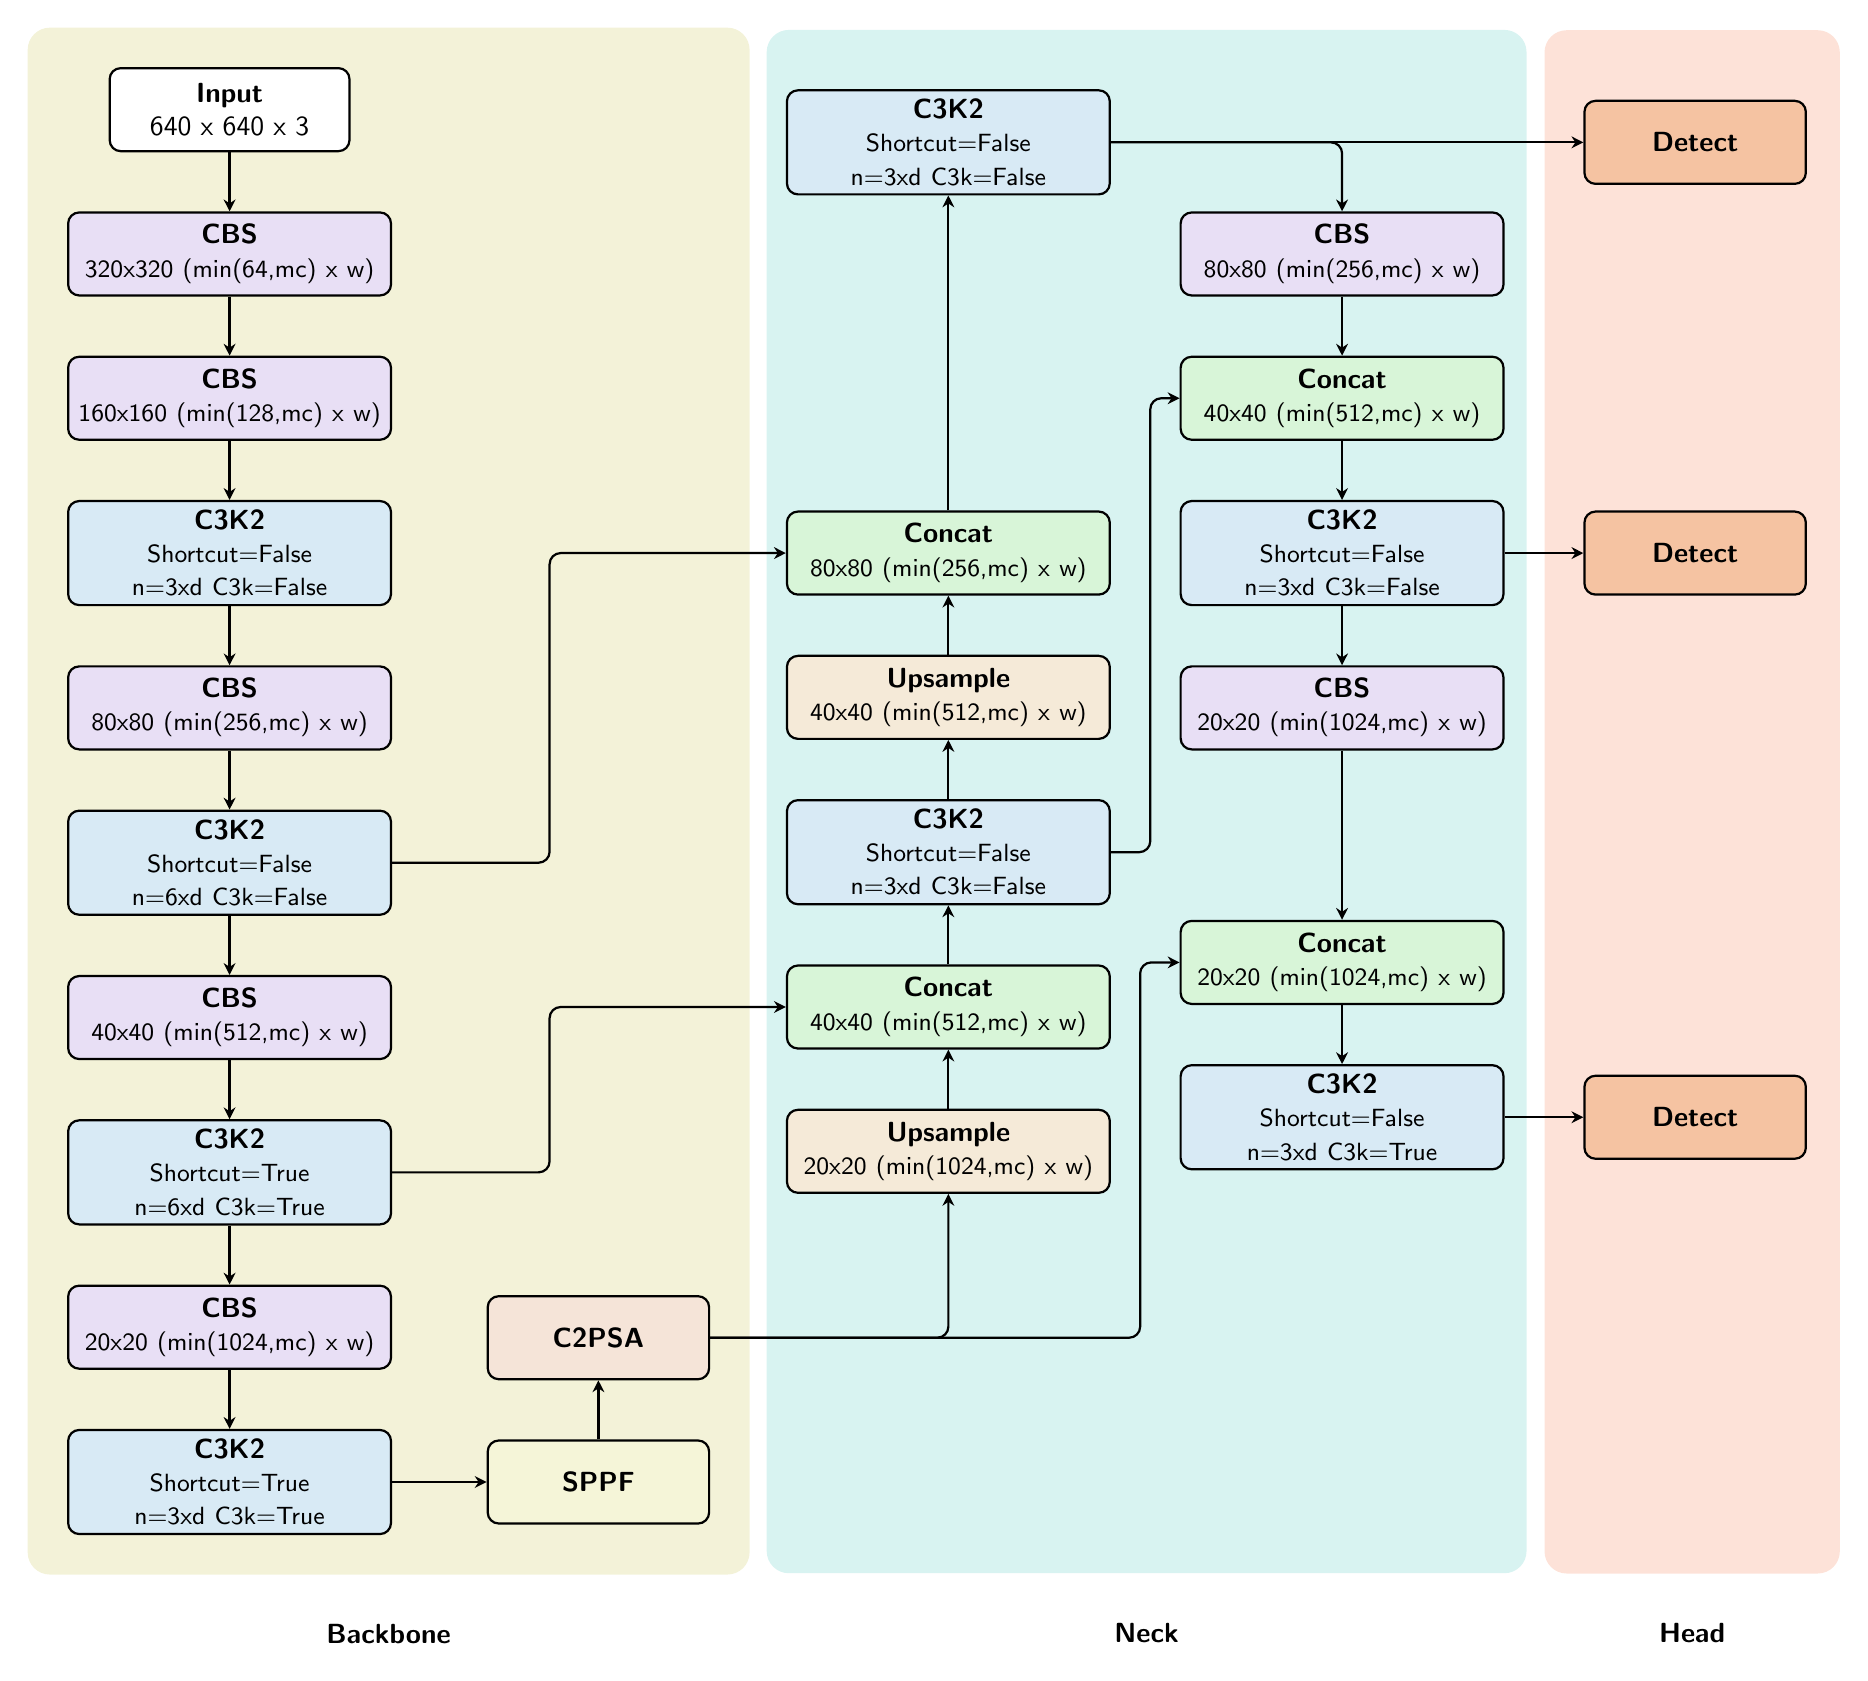
\begin{tikzpicture}[
    % Set default distances between nodes
    node distance=0.75cm and 1.2cm,
    % Define default arrow style
    >={Stealth[length=1.5mm, width=1.5mm]},
    % --- Node Styles ---
    % Base style for all blocks
    block/.style={
        rectangle,
        rounded corners=4pt,
        draw=black,
        thick,
        minimum height=3em,
        minimum width=8em,
        text centered,
        font=\sffamily
    },
    % Specific styles for each type of block, inheriting from 'block'
    input/.style={block, fill=white, text width=8em, align=center},
    conv/.style={block, fill=convcolor, text width=11em, align=center},
    c3k2/.style={block, fill=c3k2color, text width=11em, align=center},
    concat/.style={block, fill=concatcolor, , text width=11em, align=center},
    upsample/.style={block, fill=upsamplecolor, , text width=11em, align=center},
    c2psa/.style={block, fill=c2psacolor},
    sppf/.style={block, fill=sppfcolor},
    detect/.style={block, fill=detectcolor},
    % Style for the background rectangles
    bg_rect/.style={
        rectangle,
        fill=#1,
        inner sep=0.5cm,
        rounded corners=8pt
    },
    arrow_label/.style={
        font=\sffamily\footnotesize,
        midway,
        right=2pt,
        text=black
    }
]


% ==============================================================================
% ==                              NODE PLACEMENT                              ==
% ==============================================================================

% --- Column 1: Backbone ---
\node[input] (in) {\textbf{Input} \\ 640 x 640 x 3};
\node[conv, below=of in] (b_conv1) {\textbf{CBS} \\ \small 320x320 (min(64,mc) x w) };
\node[conv, below=of b_conv1] (b_conv2) {\textbf{CBS} \\ \small 160x160 (min(128,mc) x w) };
\node[c3k2, below=of b_conv2] (b_c3k2_1) {\textbf{C3K2} \\ \small Shortcut=False n=3xd C3k=False};
\node[conv, below=of b_c3k2_1] (b_conv3) {\textbf{CBS} \\ \small 80x80 (min(256,mc) x w) };
\node[c3k2, below=of b_conv3] (b_c3k2_2) {\textbf{C3K2} \\ \small Shortcut=False n=6xd C3k=False};
\node[conv, below=of b_c3k2_2] (b_conv4) {\textbf{CBS} \\ \small 40x40 (min(512,mc) x w)};
\node[c3k2, below=of b_conv4] (b_c3k2_3) {\textbf{C3K2} \\ \small Shortcut=True n=6xd C3k=True};
\node[conv, below=of b_c3k2_3] (b_conv5) {\textbf{CBS} \\ \small 20x20 (min(1024,mc) x w) };
\node[c3k2, below=of b_conv5] (b_c3k2_4) {\textbf{C3K2} \\ \small Shortcut=True n=3xd C3k=True};

% Side nodes in Backbone
\node[sppf, right=of b_c3k2_4] (sppf) {\textbf{SPPF}};
\node[c2psa, above=of sppf] (c2psa) {\textbf{C2PSA}};

% --- Column 2: Neck (Middle Column) ---
\node[concat, right= 5 cm of b_c3k2_1] (n_concat1) {\textbf{Concat} \\ \small 80x80 (min(256,mc) x w) };
\node[upsample, below=of n_concat1] (n_upsample1) {\textbf{Upsample} \\ \small 40x40 (min(512,mc) x w)};
\node[c3k2, below=of n_upsample1] (n_c3k2_2) {\textbf{C3K2} \\ \small Shortcut=False n=3xd C3k=False};
\node[concat, below=of n_c3k2_2] (n_concat2) {\textbf{Concat} \\ \small 40x40 (min(512,mc) x w)};
\node[upsample, below=of n_concat2] (n_upsample2) {\textbf{Upsample}  \\ \small 20x20 (min(1024,mc) x w)};

% --- Column 3: Neck (Right Column & Top) ---
\node[c3k2, above= 4 cm of n_concat1] (n_c3k2_top) {\textbf{C3K2} \\ \small Shortcut=False n=3xd C3k=False};
\node[conv, right= 10 cm of b_conv1] (n_conv1) {\textbf{CBS} \\ \small 80x80 (min(256,mc) x w) };
\node[concat, below=of n_conv1] (n_concat3) {\textbf{Concat} \\ \small 40x40 (min(512,mc) x w) };
\node[c3k2, below=of n_concat3] (n_c3k2_3) {\textbf{C3K2} \\ \small Shortcut=False n=3xd C3k=False};
\node[conv, below=of n_c3k2_3] (n_conv2) {\textbf{CBS} \\ \small 20x20 (min(1024,mc) x w)};
\node[concat, below= 2.15 cm of n_conv2] (n_concat4) {\textbf{Concat}  \\ \small 20x20 (min(1024,mc) x w) };
\node[c3k2, below=of n_concat4] (n_c3k2_4) {\textbf{C3K2} \\ \small Shortcut=False n=3xd C3k=True};


% --- Column 4: Head ---
\node[detect, right= 6 cm of n_c3k2_top] (h_detect1) {\textbf{Detect}};
\node[detect, right= 1 cm of n_c3k2_3] (h_detect2) {\textbf{Detect}};
\node[detect, right= 1 cm of n_c3k2_4] (h_detect3) {\textbf{Detect}};

% ==============================================================================
% ==                                 EDGES                                    ==
% ==============================================================================

% --- Backbone Connections ---
\draw[->, thick, rounded corners=4pt] (in.south) -- (b_conv1.north) ; % node[arrow_label] {640x640}
\draw[->, thick, rounded corners=4pt] (b_conv1.south) -- (b_conv2.north);
\draw[->, thick, rounded corners=4pt] (b_conv2.south) -- (b_c3k2_1.north);
\draw[->, thick, rounded corners=4pt] (b_c3k2_1.south) -- (b_conv3.north);
\draw[->, thick, rounded corners=4pt] (b_conv3.south) -- (b_c3k2_2.north);
\draw[->, thick, rounded corners=4pt] (b_c3k2_2.south) -- (b_conv4.north);
\draw[->, thick, rounded corners=4pt] (b_conv4.south) -- (b_c3k2_3.north);
\draw[->, thick, rounded corners=4pt] (b_c3k2_3.south) -- (b_conv5.north);
\draw[->, thick, rounded corners=4pt] (b_conv5.south) -- (b_c3k2_4.north);
\draw[->, thick, rounded corners=4pt] (b_c3k2_4.east) -- (sppf.west);
\draw[->, thick, rounded corners=4pt] (sppf.north) -- (c2psa.south);

% --- Backbone-to-Neck Connections ---
\draw[->, thick, rounded corners=4pt] (b_c3k2_2.east) -- ++(2,0) |- (n_concat1.west);
\draw[->, thick, rounded corners=4pt] (b_c3k2_3.east) -- ++(2,0) |- (n_concat2.west);
\draw[->, thick, rounded corners=4pt] (c2psa.east) -- ++ (1,0) -| (n_upsample2.south);
\draw[->, thick, rounded corners=4pt] (c2psa.east) -- ++(0.5,0) -| ($(n_concat4.west)+(-0.5,0)$) -- (n_concat4.west);


% (n_concat4.west)

% --- Neck Internal Connections ---
% Upward flow in the middle column
\draw[->, thick, rounded corners=4pt] (n_upsample2.north) -- (n_concat2.south);
\draw[->, thick, rounded corners=4pt] (n_concat2.north) -- (n_c3k2_2.south);
\draw[->, thick, rounded corners=4pt] (n_c3k2_2.north) -- (n_upsample1.south);
\draw[->, thick, rounded corners=4pt] (n_upsample1.north) -- (n_concat1.south);
\draw[->, thick, rounded corners=4pt] (n_concat1.north) -- (n_c3k2_top.south);

% Downward flow in the right column
% \draw[->] (n_c3k2_top.east) -- ++(0.5,0) |- (n_conv1.north);
\draw[->, thick, rounded corners=4pt] (n_conv1.south) -- (n_concat3.north);
\draw[->, thick, rounded corners=4pt] (n_concat3.south) -- (n_c3k2_3.north);
\draw[->, thick, rounded corners=4pt] (n_c3k2_3.south) -- (n_conv2.north);
\draw[->, thick, rounded corners=4pt] (n_conv2.south) -- (n_concat4.north);
\draw[->, thick, rounded corners=4pt] (n_concat4.south) -- (n_c3k2_4.north);

% Connections from middle to right column
\draw[->, thick, rounded corners=4pt] (n_c3k2_2.east) -- ++(0.5,0) |- (n_concat3.west);
\draw[->, thick, rounded corners=4pt] (n_c3k2_top.east) -- ++(0.5, 0) -| (n_conv1.north);

% --- Neck-to-Head Connections ---
\draw[->, thick, rounded corners=4pt] (n_c3k2_top.east) -- (h_detect1.west);
\draw[->, thick, rounded corners=4pt] (n_c3k2_3.east) -- (h_detect2.west);
\draw[->, thick, rounded corners=4pt] (n_c3k2_4.east) -- (h_detect3.west);


% ==============================================================================
% ==                         BACKGROUNDS AND LABELS                           ==
% ==============================================================================

% Use the 'on background layer' to draw elements behind everything else
\begin{scope}[on background layer]
    % Create nodes that fit around the components of each section
    \node[bg_rect=backbonebg, fit=(in) (b_c3k2_4) (c2psa)] (backbone_bg) {};
    
    \node[bg_rect=neckbg, minimum width=9.65cm, minimum height=19.6cm, anchor=north west, yshift=0.76cm, xshift=-0.25cm] at (n_c3k2_top.north west) (neck_bg) {};
    
    \node[
    bg_rect=headbg,
    minimum width=3.75cm,
    minimum height=19.6cm,
    anchor=north west,
    yshift=0.89cm,
    xshift=-0.5cm
    ] at (h_detect1.north west) (head_bg) {};

\end{scope}


% Add labels below the background boxes
\node[below=0.5cm of backbone_bg.south, font=\sffamily\bfseries] {Backbone};
\node[below=0.5cm of neck_bg.south, font=\sffamily\bfseries] {Neck};
\node[below=0.5cm of head_bg.south, font=\sffamily\bfseries] {Head};

\end{tikzpicture}
\end{document}